
%\documentclass[letterpaper, 10 pt, conference]{ieeeconf}  % Comment this line out
                                                          % if you need a4paper
\documentclass[a4paper, 10pt, conference]{ieeeconf}      % Use this line for a4
                                                          % paper
                                                          
\IEEEoverridecommandlockouts                              % This command is only
                                                          % needed if you want to
                                                          % use the \thanks command
\overrideIEEEmargins
\usepackage{graphics} % for pdf, bitmapped graphics files


\begin{document}
\begin{figure}[htbp]
    \centering
    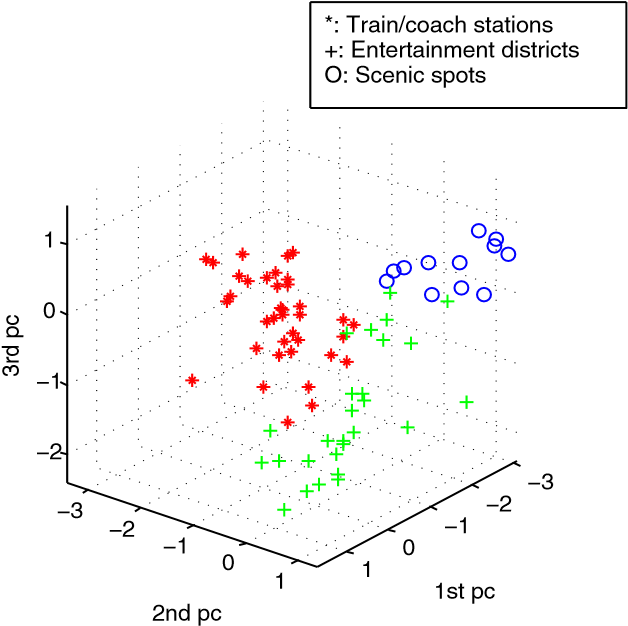
\includegraphics{fig/f6.png}
    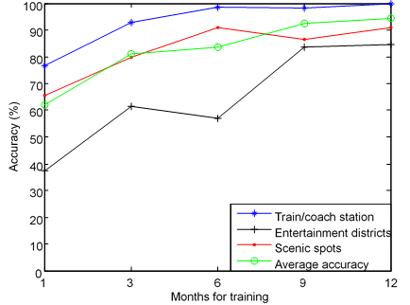
\includegraphics{fig/f7.png}
    \caption{}
    \label{fig:my_label}
\end{figure}

\begin{equation}
\label{eq:one}
\ut - \alpha \uxx + \beta (u-u_{air}) + \gamma (u^4 - u_{air}^4)  = 0.
\end{equation} 

\begin{equation}
\label{eq:two}
\ut - \alpha\uxx = 0.
\end{equation}
\begin{equation}
\label{eq:three}
\Qt = -\kappa A_{\times}\frac{du}{dx}.
\end{equation}

\begin{equation}
\label{eq:four}
\frac{dQ_{net}}{dt} = (c_{Al}\rho dV) u_{rise}.
\end{equation}


\begin{equation}
    x=\frac{-b\pm\sqrt{b^2-4ac}}{2a}.
    \label{eq:quadratic}
\end{equation}

$$    x=\frac{-b\pm\sqrt{b^2-4ac}}{2a}.
    \label{eq:quadratic}
$$

\end{document}